\label{sec:splitting-timing}
Figure \ref{fig:comparison_efficiency} shows comparison of the parallel efficiency of the RMSD task between different test cases on SDSC Comet.  

\begin{figure}[ht!]
\centering
  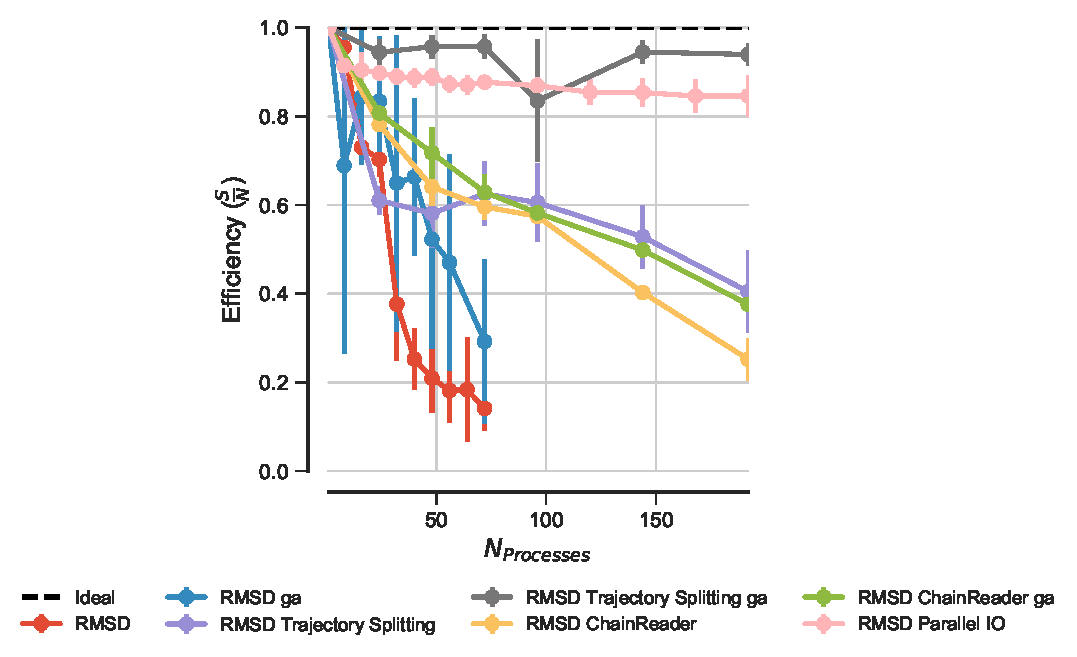
\includegraphics[width=0.65\linewidth]{figures/Comparison_Efficiency_all.pdf}
\caption{Comparison of the parallel efficiency between different test cases on SDSC Comet.
Five repeats were performed to collect statistics and error bars show standard deviation with respect to mean.}
\label{fig:comparison_efficiency}
\end{figure} 

Figure \ref{fig:MPIwithIO-split-SuperMIC} shows how RMSD task scales with the increase in the number of cores when the trajectories are split using GA and without GA on SuperMIC.  
 
 \begin{figure}[ht!]
\centering
\begin{subfigure}{.3\textwidth}
  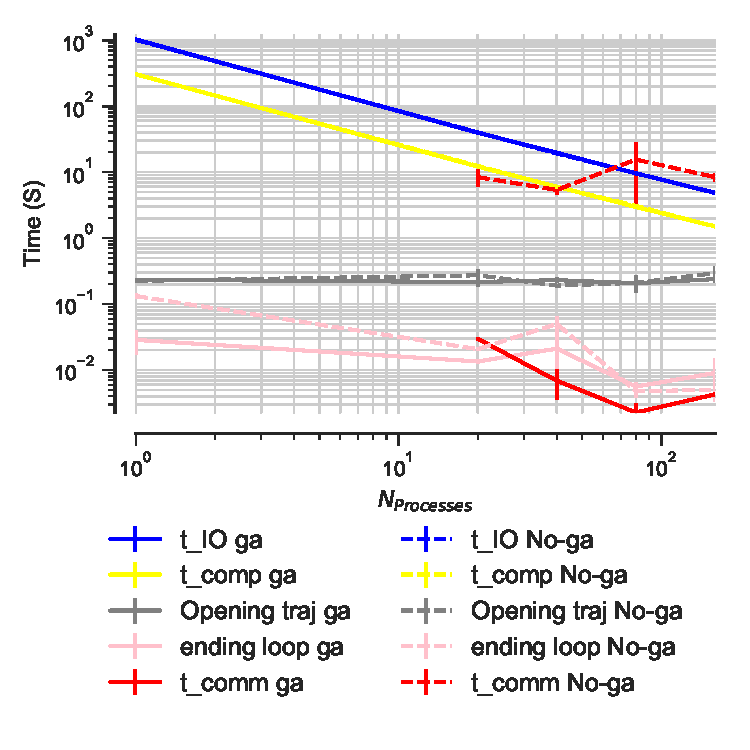
\includegraphics[width=\linewidth]{figures/Comparison_IO_compute_scaling_traj_splitting-SuperMIC.pdf}
  \caption{Scaling for different components}
  \label{fig:MPIscaling-chain-reader}
\end{subfigure}
\hfill
\begin{subfigure}{.3\textwidth}
  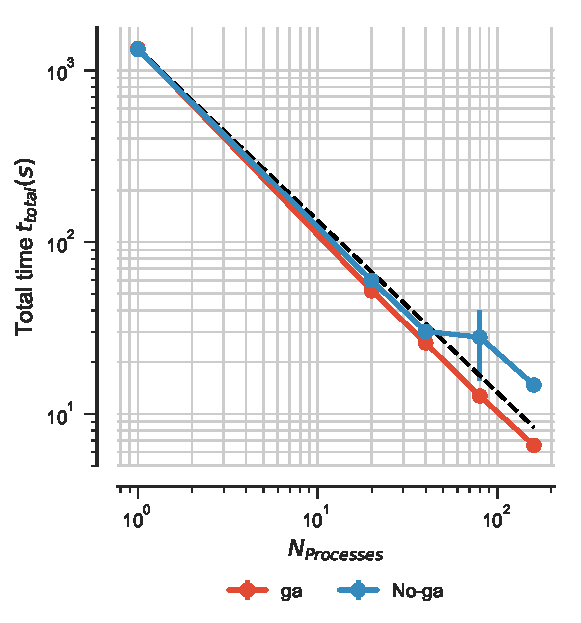
\includegraphics[width=\linewidth]{figures/Comparison_tot_time_traj_splitting-SuperMIC.pdf}
  \caption{Scaling total}
  \label{fig:MPItottime-chain-reader}
\end{subfigure}
\hfill
\begin{subfigure}{.3\textwidth}
  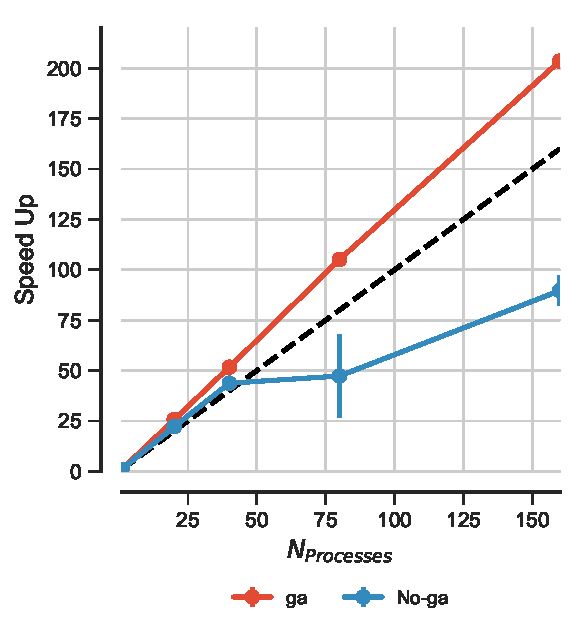
\includegraphics[width=\linewidth]{figures/Comparison_Speed_UP_traj_splitting-SuperMIC.pdf}
  \caption{Speed-up}
  \label{fig:MPIspeedup-chain-reader}
\end{subfigure}

\caption{Comparison on the performance of the RMSD task with MPI when the trajectories are split using global array and without global array ($\tcomp/\tIO \approx 0.3$) on SuperMIC.
In case of global array, all ranks update the global array (\text{$ga_{\text{put}}$}) and rank 0 accesses the whole RMSD array through the global memory address (\text{$ga_{\text{get}}$}).
Five repeats were performed to collect statistics. (a) Compute \& I/O scaling versus number of processes (b) Total time scaling versus number of processes (c) Speed-up (a-c) The error bars show standard deviation with respect to mean.}
\label{fig:MPIwithIO-split-SuperMIC}
\end{figure}


We ran a benchmark where no I/O was performed and instead generated random input data of the same size as would have been obtained from the trajectory; the time for the data generation was excluded and no file access was necessary. 
In this case, we observed rather good scaling behavior with communication effect being less pronounced (Figure \ref{fig:MPIwithoutIO}).


 \begin{figure}[ht!]
\centering
\begin{subfigure}{.35\textwidth}
  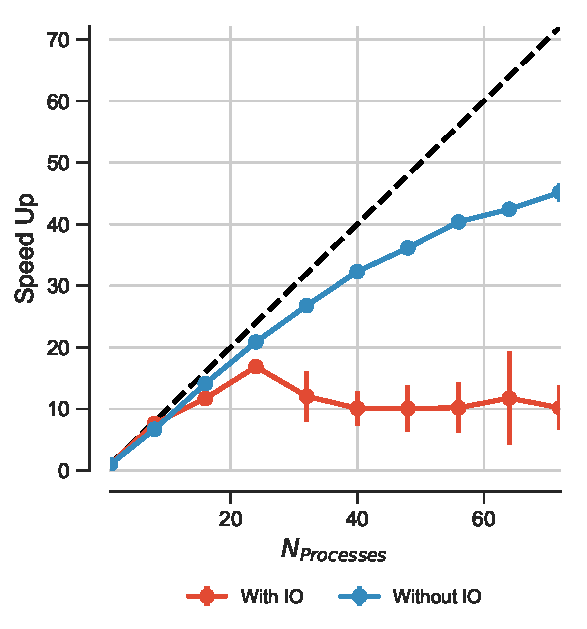
\includegraphics[width=\linewidth]{figures/speed_up-effect-of-IO.pdf}
  \caption{Speed up comparison}
  \label{fig:MPIspeedup-no-IO}
\end{subfigure}
\hfill
\begin{subfigure}{.5\textwidth}
  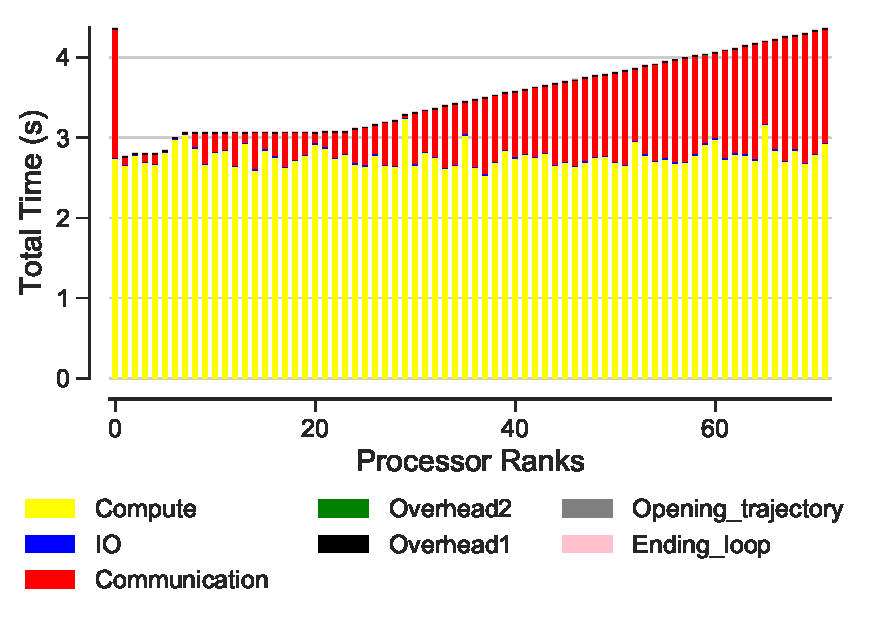
\includegraphics[width=\linewidth]{figures/BarPlot-rank-comparison-no-IO.pdf}
  \caption{Time comparison on different parts of the calculations per MPI rank when I/O is removed}
  \label{fig:MPIranks-no-IO}
\end{subfigure}

\caption{Comparison on the performance of RMSD task with MPI with I/O and without I/O ($\tcomp/\tIO \approx 0.3$) on SDSC Comet.
Five repeats were performed to collect statistics. (a) Speed-up. The error bars show standard deviation with respect to mean.
(b) Compute \tcomp, IO \tIO, communication \tcomm, ending the for loop \text{$t_{\text{end\_loop}}$},
  opening the trajectory \text{$t_{\text{opening\_trajectory}}$}, and overheads \text{$t_{\text{overhead1}}$}, \text{$t_{\text{overhead2}}$} per MPI rank (See Table \ref{tab:notation} for the definition).}
\label{fig:MPIwithoutIO}
\end{figure}
